\AgdaHide{ \begin{code}

open import base

module EarleysAlgorithm (N T : Set) (eqₙ : Dec N) (eqₜ : Dec T) where

open import grammar-mini N T
\end{code}}
\chapter{Earley's Algorithm} \label{Earleys}

	The Earley parsing algorithm, named after its inventor Jay Earley, was
	first described in 1968~\cite{Earley}. It is a top-down parsing algorithm,
	meaning that it starts with analyzing the large-scale structure of its
	input and uses that as guidance for what analysis is needed when diving
	deeper into more fine-grain structure and eventually single tokens.  Earley
	parsing is interesting in that it is able to perform well on several
	commonly used types of grammars, such as the grammars parseable by LR
	parsers, while also being able to parse all context-free grammars. This
	section will first give a high-level description of the algorithm, followed
	by a formalization of its mechanics, and finally describe our
	implementation of the algorithm in Agda.

	\section{Description}

		The Earley algorithm works by keeping track of a set of items
		representing possible partial parses for each position in the input
		sequence. It advances over the sets from left to right, with each step
		to the right representing the consumption, or \emph{`scanning'} of one
		token. When completing a set, all items generated by scanning from
		the previous set are first analyzed to determine if any further action
		can be taken on any of them that will generate new items. All new items
		are then added into the set (or, when doing scanning, to the next set),
		and all new items in the current set are then analyzed to determine
		if any new items can be constructed. This is repeated until there are
		no more items to create, and the process then continues to the next
		item set.

		The items are of the form $\earley{X}{\alpha}{\beta}{i}$, where $X$ is
		the non-terminal that was being analyzed when this item was created,
		$\alpha$ is the sequence of terminals and non-terminals that have
		already been successfully parsed, $\beta$ is what remains to be parsed,
		and $i$ is the index of the set where the parsing attempt of $X$ was
		started. We will use $\St{i}$ to mean the item set at position $i$,
		between character $i$ and $i+1$. New items can be constructed from
		previous items in three ways:

		\begin{itemize}
			\item

				If $\beta$ is of the form $Y\delta$, meaning that for this item
				to be completed, a $Y$ must now be parsed at this position, all
				items on the form $\earley{Y}{\epsilon}{\gamma}{j}$, where $j$
				is the current position, are added to the current set. We call
				this to \emph{predict} based on the current item.

			\item

				If $\beta$ is of the form $\epsilon$, meaning that this item
				could accept the string of tokens starting at $i$ and ending at
				the current position, $j$, we must find out why the parsing of
				$X$ was attempted in the first place. Any item
				$\earley{Y}{\alpha}{X\delta}{k}$ in set $i$  could have
				predicted this item, and as such, we will add a new item
				$\earley{Y}{\alpha X}{\delta}{k}$ for each such item to the
				current item set, $S_j$. We call this to \emph{complete} the
				current item.

			\item

				If $\beta$ is of the form $a\delta$, and the next token in the
				input sequence is $a$, a new item $\earley{X}{\alpha
				a}{\delta}{i}$ is added to the next set. We call this to
				\emph{scan} the current item.

		\end{itemize}

		The algorithm is initialized with all sets empty except for the first
		one, where a single item $\earley{S_0}{\epsilon}{S}{0}$ is inserted.
		$S$ is the starting symbol, that is, the non-terminal which we want to
		find out if the input sequence conforms to or not. $S_0$ is a special
		marker that is only used for the initial item. When parsing of the
		input sequence is complete, if in the last set there is an item
		$\earley{S_0}{S}{\epsilon}{0}$ then the parser accepts, otherwise the
		parser rejects the input.

		The parse tree can be constructed via backtracking from the item
		sets. The nifty thing about this algorithm is that since each item can only
		exist once in each item set, if the grammar is ambiguous and items can
		be derived in several different ways (or even an unbounded number of
		ways), the different derivations will all share their common items,
		which gives the Earley parsing algorithm the ability to correctly
		analyze ambiguous grammars efficiently.

	\section{An Example}

		%\todo{I guess an example of an Earley parser run would be helpful in
		%this section. (And in your thesis defense!)}

		To get a clear understanding of how the Earley parsing algorithm works,
		we will use it to analyze a short string with a simple grammar. The
		grammar rules are as follows:

		\begin{table}[h]
		\centering
		\begin{tabular}{rcl}
			$E$ & $ \mapsto $ & $V$ \\
			$E$ & $ \mapsto $ & $E$ $O$ $E$ \\
			$O$ & $ \mapsto $ & $+$ \\
			$O$ & $ \mapsto $ & $-$ \\
			$V$ & $ \mapsto $ & $x$ \\
			$V$ & $ \mapsto $ & $y$ \\
			$V$ & $ \mapsto $ & $z$
		\end{tabular}
		\end{table}

		We will take $E$ to be the starting symbol of the grammar, and we will
		attempt to parse the string ``$x+y$''. First, we prepare the parser
		state by creating four empty sets, and adding the initial item to the
		first one:

%		\todo{Is it necessary to add a new starting symbol $S_0$?  Couldn't you
%		use $E$ as you do in the Agda formalization?  This would amount to
%		adding all rules for $E$ as initial rules, and accept an input as soon
%		as one of the rules for $E$ added in state $0$ has been completed.}

		\begin{table}[h]
		\centering
		\begin{tabular}{|c|c|c|c|}
			\hline
			$\St{0}$ & $\St{1}$ & $\St{2}$ & $\St{3}$ \\
			\hline
			$\earley{S_0}{\varepsilon}{E}{0}$ & & & \\
			\hline
		\end{tabular}
		\end{table}

		Now we start working on the first item set, $\St{0}$. The first, and
		only, item in that set can be used to predict two new items,
		yielding the items $\earley{E}{\varepsilon}{V}{0}$ and
		$\earley{E}{\varepsilon}{EOE}{0}$. These two are then added to
		$\St{0}$:

		\begin{table}[h]
		\centering
		\begin{tabular}{|c|c|c|c|}
			\hline
			$\St{0}$ & $\St{1}$ & $\St{2}$ & $\St{3}$ \\
			\hline
			$\earley{S_0}{\varepsilon}{E}{0}$ & & & \\
			$\earley{E}{\varepsilon}{V}{0}$   & & & \\
			$\earley{E}{\varepsilon}{EOE}{0}$ & & & \\
			\hline
		\end{tabular}
		\end{table}

		The first of these new items, now item number two in $\St{0}$, can also
		be used for predicting new items, yielding
		$\earley{V}{\varepsilon}{x}{0}$ , $\earley{V}{\varepsilon}{y}{0}$, and
		$\earley{V}{\varepsilon}{z}{0}$.  The item at position three can also
		be used for prediction, but as all results of that prediction are
		already in $\St{0}$, nothing happens. The three new items added from
		rule three can all be scanned, but only one of them match our input
		string, yielding the following state:

		\begin{table}[h]
		\centering
		\begin{tabular}{|c|c|c|c|}
			\hline
			$\St{0}$                          & $\St{1}$ & $\St{2}$ & $\St{3}$ \\
			\hline
			$\earley{S_0}{\varepsilon}{E}{0}$ & $\earley{V}{x}{\varepsilon}{0}$ & &\\
			$\earley{E}{\varepsilon}{V}{0}$   & & & \\
			$\earley{E}{\varepsilon}{EOE}{0}$ & & & \\
			$\earley{V}{\varepsilon}{x}{0}$   & & & \\
			$\earley{V}{\varepsilon}{y}{0}$   & & & \\
			$\earley{V}{\varepsilon}{z}{0}$   & & & \\
			\hline
		\end{tabular}
		\end{table}

		Now there is nothing to be done with any of the items in $\St{0}$, and
		so we move on to $\St{1}$. The first item here can be completed. Since
		it has index $0$, we will look in $\St{0}$ for matching items to
		complete with. The second item matches, and so we add a new item
		$\earley{E}{V}{\varepsilon}{0}$ to the current set $\St{1}$. This new
		item can also be completed, and also has index $0$, with two matching
		items in $\St{0}$:

		\begin{table}[h]
		\centering
		\begin{tabular}{|c|c|c|c|}
			\hline
			$\St{0}$                          & $\St{1}$ & $\St{2}$ & $\St{3}$ \\
			\hline
			$\earley{S_0}{\varepsilon}{E}{0}$ & $\earley{V}{x}{\varepsilon}{0}$   &  & \\
			$\earley{E}{\varepsilon}{V}{0}$   & $\earley{E}{V}{\varepsilon}{0}$   &  & \\
			$\earley{E}{\varepsilon}{EOE}{0}$ & $\earley{S_0}{E}{\varepsilon}{0}$ &  & \\
			$\earley{V}{\varepsilon}{x}{0}$   & $\earley{E}{E}{OE}{0}$            &  & \\
			$\earley{V}{\varepsilon}{y}{0}$   &                                   &  & \\
			$\earley{V}{\varepsilon}{z}{0}$   &                                   &  & \\
			\hline
		\end{tabular}
		\end{table}

		At this point, we have completed the initial item, meaning that we
		could accept this input if it ended here. Since there is more input to
		parse, we continue with using item four for predicting more items. When
		we are done with $\St{1}$ our state looks like this:

		\begin{table}[H]
		\centering
		\begin{tabular}{|c|c|c|c|}
			\hline
			$\St{0}$                          & $\St{1}$                          &$\St{2}$ & $\St{3}$ \\
			\hline
			$\earley{S_0}{\varepsilon}{E}{0}$ & $\earley{V}{x}{\varepsilon}{0}$   & $\earley{O}{+}{\varepsilon}{1}$ & \\
			$\earley{E}{\varepsilon}{V}{0}$   & $\earley{E}{V}{\varepsilon}{0}$   & & \\
			$\earley{E}{\varepsilon}{EOE}{0}$ & $\earley{S_0}{E}{\varepsilon}{0}$ & & \\
			$\earley{V}{\varepsilon}{x}{0}$   & $\earley{E}{E}{OE}{0}$            & & \\
			$\earley{V}{\varepsilon}{y}{0}$   & $\earley{O}{\varepsilon}{+}{1}$   & & \\
			$\earley{V}{\varepsilon}{z}{0}$   & $\earley{O}{\varepsilon}{-}{1}$   & & \\
			\hline
		\end{tabular}
		\end{table}

		Continuing to add items all the way until the end we get the following
		state:

		\begin{table}[h]
		\centering
		\begin{tabular}{|c|c|c|c|}
			\hline
			$\St{0}$                          & $\St{1}$                          & $\St{2}$                         $ & $\St{3}$ \\
			\hline
			$\earley{S_0}{\varepsilon}{E}{0}$ & $\earley{V}{x}{\varepsilon}{0}$   & $\earley{O}{+}{\varepsilon}{1}  $ & $\earley{V}{y}{\varepsilon}{2}  $ \\
			$\earley{E}{\varepsilon}{V}{0}$   & $\earley{E}{V}{\varepsilon}{0}$   & $\earley{E}{EO}{E}{0}           $ & $\earley{E}{V}{\varepsilon}{2}  $ \\
			$\earley{E}{\varepsilon}{EOE}{0}$ & $\earley{S_0}{E}{\varepsilon}{0}$ & $\earley{E}{\varepsilon}{V}{2}  $ & $\earley{E}{EOE}{\varepsilon}{0}$ \\
			$\earley{V}{\varepsilon}{x}{0}$   & $\earley{E}{E}{OE}{0}$            & $\earley{E}{\varepsilon}{EOE}{2}$ & $\earley{E}{E}{OE}{2}           $ \\
			$\earley{V}{\varepsilon}{y}{0}$   & $\earley{O}{\varepsilon}{+}{1}$   & $\earley{V}{\varepsilon}{x}{2}  $ & $\earley{E}{E}{OE}{0}           $ \\
			$\earley{V}{\varepsilon}{z}{0}$   & $\earley{O}{\varepsilon}{-}{1}$   & $\earley{V}{\varepsilon}{y}{2}  $ & $\earley{S_0}{E}{\varepsilon}{0}$ \\
			$                                 &                                   & $\earley{V}{\varepsilon}{z}{2}  $ & $\earley{O}{\varepsilon}{+}{3}  $ \\
			$                                 &                                   &                                 $ & $\earley{O}{\varepsilon}{-}{3}  $ \\
			\hline
		\end{tabular}
		\end{table}

		Since the item $\earley{S_0}{E}{\varepsilon}{0}$ is in $\St{3}$ the
		input sequence is in the grammar, and we accept the input. We can work
		our way backwards from this item using the construction rules in
		reverse to figure out how it was made and construct a parse tree for
		it.

	\section{Formalization}

		We will begin by defining a proposition for how and what items can be
		added to the different sets.

		\begin{table}[h]
			\centering
			\begin{tabular}{cc}
				\( \displaystyle \frac{}
					{\earley{S_0}{\epsilon}{S}{0} \in \St{0}}
					~~\textrm{start } S
					\) &
				\( \displaystyle \frac
					{\earley{X}{\alpha}{Y\beta}{i} \in \St{j}}
					{\earley{Y}{\epsilon}{\delta}{j} \in \St{j}}
					~~Y \mapsto \delta
					\)
				\\~&~\\
				\( \displaystyle \frac
					{\earley{X}{\alpha}{a\beta}{i} \in \St{j}}
					{\earley{X}{\alpha a}{\beta}{i} \in \St{j+1}}
					\textrm{next-char } a 
					\) &
				\( \displaystyle \frac
					{
						\earley{X}{\alpha}{Y\beta}{i} \in \St{j}~~~~
						\earley{Y}{\gamma}{\epsilon}{j} \in \St{k}
						}
					{\earley{X}{\alpha Y}{\beta}{i} \in \St{k}}
					\)
			\end{tabular}
		\end{table}

%		\todo{The Agda formalization does not have $S_0$; thus, a better match
%		would be the start rule $\earley S \epsilon \alpha 0 \in \St 0$ where
%		$S \mapsto \alpha$ is a grammar rule for start symbols $S$.}

		These inference rules match closely with the descriptions of how new
		items can be constructed, together with the initial item, and a similar
		proposition can be constructed in Agda:

		\AgdaHide{\begin{code}
			infixl 10 _∙_⊢_/_⟶*_/_∙_
		\end{code}}
		\begin{code}
			data _∙_⊢_/_⟶*_/_∙_ (G : CFG) (input : T *) :
			  (u v : T *) → N → (N ∣ T) * → (N ∣ T) * → Set where

			  initial : {α : (N ∣ T) *} →
			    (CFG.start G , α) ∈ CFG.rules G →
			    G ∙ input ⊢ input / input ⟶* CFG.start G / ε ∙ α

			  scanner : {u v : T *} {a : T} {X : N} {α β : (N ∣ T) *} →
			    G ∙ input ⊢ u / a ∷ v ⟶* X / α ∙ (r a ∷ β) →
			    G ∙ input ⊢ u / v ⟶* X / (α ←∷ r a) ∙ β

			  predict : {u v : T *} {X Y : N} {α β δ : (N ∣ T) *} →
			    CFG.rules G ∋ (Y , δ) →
			    G ∙ input ⊢ u / v ⟶* X / α ∙ (l Y ∷ β) →
			    G ∙ input ⊢ v / v ⟶* Y / ε ∙ δ

			  complet : {u v w : T *} {X Y : N} {α β γ : (N ∣ T) *} →
			    G ∙ input ⊢ u / v ⟶* X / α ∙ (l Y ∷ β) →
			    G ∙ input ⊢ v / w ⟶* Y / γ ∙ ε →
			    G ∙ input ⊢ u / w ⟶* X / (α ←∷ l Y) ∙ β
		\end{code}
		\AgdaHide{\begin{code}
			in-g : ∀ {G t u v X α β} →
			  G ∙ t ⊢ u / v ⟶* X / α ∙ β →
			    CFG.rules G ∋ (X , α ++ β)
			in-g (initial x) = x
			in-g (scanner g) = in₂ (λ t → (_ , t) ∈ _) (in₀ _ _ _) (in-g g)
			in-g (predict x g) = x
			in-g (complet g g₁) = in₂ (λ t → (_ , t) ∈ _) (in₀ _ _ _) (in-g g)

			suff-g₃ : ∀ {G t u v X α β} →
			  G ∙ t ⊢ u / v ⟶* X / α ∙ β →
			    Σ λ s → s ++ v ≡ u
			suff-g₃ (initial x) = σ ε refl
			suff-g₃ (scanner g) with suff-g₃ g
			suff-g₃ (scanner {a = a} g) | σ p₁ p₀ = σ (p₁ ←∷ a) (trans (sym (in₀ _ _ _)) (sym p₀))
			suff-g₃ (predict x g) = σ ε refl
			suff-g₃ (complet g g₁) with suff-g₃ g , suff-g₃ g₁
			suff-g₃ (complet g g₁) | σ p₁ p₀ , σ q₁ q₀ =
			  σ (p₁ ++ q₁) (trans (trans (assoc-++ p₁ _ _) (app (p₁ ++_) (sym q₀))) (sym p₀))

			suff-g₂ : ∀ {G t u v X α β} →
			  G ∙ t ⊢ u / v ⟶* X / α ∙ β →
			    Σ λ s → s ++ v ≡ t
			suff-g₂ (initial x) = σ ε refl
			suff-g₂ (predict x g) = suff-g₂ g
			suff-g₂ (complet g g₁) = suff-g₂ g₁
			suff-g₂ (scanner g) with suff-g₂ g
			suff-g₂ (scanner {a = a} g) | σ p₁ p₀ =
			  σ (p₁ ←∷ a) let x₁ = in₀ a p₁ _ in trans (sym x₁) (sym p₀)

			suff-g₁ : ∀ {G t u v X α β} →
			  G ∙ t ⊢ u / v ⟶* X / α ∙ β →
			    Σ λ s → s ++ u ≡ t
			suff-g₁ (initial x) = σ ε refl
			suff-g₁ (scanner g) = suff-g₁ g
			suff-g₁ (predict x g) = suff-g₂ g
			suff-g₁ (complet g g₁) = suff-g₁ g

		\end{code}}
		We use the notation \codett{α ←∷ r a} for appending \codett{r a} to the
		end of \codett{α}.

\newcommand{\tdrop}{\mathsf{drop}}
\newcommand{\tlength}{\mathsf{length}}
\newcommand{\vinput}{\mathit{input}}
\newcommand{\rslash}{\mathrel{{}/{}}}


		A value with type $G \cdot \vinput \vdash u \rslash v \rightarrow^* X
		\rslash \alpha \cdot \beta$ can be thought of as corresponding to an
		item $\earley{X}{\alpha}{\beta}{u} \in \St{v}$. However, the Agda
		version uses $u$ and $v$ as remainders of the input string rather than
		indicies into it.  Given an Earley item {$\earley{X}{\alpha}{\beta}{i}
		\in \St{j}$, the corresponding type for the data type in Agda would then
		be $G \cdot \vinput \vdash (\tdrop\;i\;\vinput) \rslash
		(\tdrop\;j\;\vinput) \rightarrow^* X \rslash \alpha \cdot \beta$, where
		$\tdrop$ removes a specified number of elements from a list. Going the
		other way, $G \cdot \vinput \vdash u \rslash v \rightarrow^* X \rslash
		\alpha \cdot \beta$ would correspond to an Earley item
		$\earley{X}{\alpha}{\beta}{n - \tlength\;u} \in \St{n - \tlength\;v}$},
		where $\tlength$ returns the number of elements in a list and $n =
		\tlength\;\vinput$.

		There are some other differences between the propositions we first
		wrote for Earley parsers and the data type given above. The addition of
		an explicit grammar and input sequence change little about the how the
		constructors can be used, but make it easier to reason about different
		grammars and ensure that the initial item will indeed only be put in
		the initial item set. The initial item has also been changed somewhat.
		Instead of introducing a special marker for the initial item, all rules
		for the starting symbol are now allowed as initial items.  This also
		has little effect on the propositions, but introduces a useful
		invariant: $X \mapsto \alpha \concat \beta \in \textsf{rules } G$.

		We also provide proofs that these propositions are sound and complete
		with respect to the parsing propositions provided in
		Chapter~\ref{Parsing}:

		\begin{code}
			sound₁ : ∀ {G t u v w X α β} →
			  G ∙ t ⊢ u / v ⟶* X / α ∙ β →
			    G ⊢ v ∥ w ∈ β →
			    G ⊢ u ∥ w ∈ α ++ β
			sound₁ (initial x)     b = b
			sound₁ (scanner g)     b = sound₁ g (term b)
			sound₁ (predict x g)   b = b
			sound₁ (complet g g₁)  b =
			  let b₁ = (sound₁ g₁ empt) in
			  let x₁ = (in-g g₁) in
			  let b₂ = conc x₁ b₁ b in
			  (sound₁ g b₂)
		\end{code}
		
%		\todo{Consider using different letters than $x$.  In particular,
%		elements different types should be represented by different letters.
%		E.g., you could use $r$ for rules, $d$ for Earley derivations etc.
%		This helps with reading these proofs.}

		Soundness is fairly straightforward. The \codett{in-g} function proves
		the invariant $\alpha \concat \beta \in \textsf{rules } G$ for the
		Earley propositions. The function as shown here is not entirely
		complete: there are several instances of string concatenation that do
		not disappear during normalization, but these are not directly relevant
		to the proof at hand. Completeness follows in a similar fashion:

		\begin{code}
			complete₁ : ∀ {t u v w X α β} {G : CFG} →
			  G ∙ t ⊢ u / v ⟶* X / α ∙ β →
			    G ⊢ v ∥ w ∈ β →
			  G ∙ t ⊢ u / w ⟶* X / α ++ β ∙ ε
			complete₁ b empt = b
			complete₁ b (conc x g g₁) =
			  let b₁ = predict x b in
			  let b₂ = complete₁ b₁ g in
			  let g₂ = complet b b₂ in
			  let g₃ = complete₁ g₂ g₁ in
			  g₃
			complete₁ b (term g) =
			  let g' = complete₁ (scanner b) g in
			  g'
		\end{code}

		Like with the soundness proof some parts related to string
		concatenation equalities have been elided. Being both sound and
		complete, we expect the propositions we have given for Earley parsing
		to be reasonable enough to be useful for proving the correctness of an
		implementation of the algorithm. The close similarities between the
		constructors for the Earley propositions and the steps in the algorithm
		itself will also make it easier to show these properties for an
		implementation.

	\section{Implementation}
		\AgdaHide{\begin{code}
			module parser (G : CFG) where
			  open import count N T eqₙ eqₜ

			  v-step : ∀ {Y α x β} →
			    CFG.rules G ∋ (Y , α ++ (x ∷ β)) → CFG.rules G ∋ (Y , (α ←∷ x) ++ β)
			  v-step {Y} {α} {x} {β} v =
			    in₂ (λ x → CFG.rules G ∋ (Y , x)) (in₀ x α β) v

			  v-unstep : ∀ {Y α x β} →
			    CFG.rules G ∋ (Y , (α ←∷ x) ++ β) → CFG.rules G ∋ (Y , α ++ (x ∷ β))
			  v-unstep {Y} {α} {x} {β} v =
			    in₂ (λ x → CFG.rules G ∋ (Y , x)) (sym (in₀ x α β)) v
		\end{code}}

		We start by creating a representation for the Earley items:

		\begin{code}
			  record Item (w : T *) (v : T *) : Set where
			    constructor _∘_↦_∘_
			    field
			      Y : N
			      u : T *
			      α β : (N ∣ T) *
			      .{χ} : CFG.rules G ∋ (Y , α ++ β)
			      .{ψ} : (Σ λ t → t ++ u ≡ w)        -- u is a suffix of w
		\end{code}

		Here, $Y \circ u \mapsto \alpha \circ \beta : \textrm{Item } w\ v$
		represents an Earley item $\earley{Y}{\alpha}{\beta}{u}$ that was
		generated when parsing the input sequence $w$ up to, but not including,
		the remainder $v$. Each item also carries with it a proof that it
		matches some rule in the grammar ($\psi$), as well as a proof that the
		index $u$ fits somewhere in the entire sequence $w$ ($\chi$). These
		proofs are declared irrelevant which means that they must be part of
		every item, but are not considered part of the data type for e.g.
		propositional equality, since we only care that the validity proofs
		exist not that equal items must have equal validity proofs (although
		they likely will). We could also have provided the invariant of $v$
		being a suffix of $u$, or $v$ of $w$, but these were not used in our
		implementation or proofs.

		\AgdaHide{\begin{code}
			  infixl 3 _∘_↦_∘_
			  pattern _∘_↦_∘_[_∘_] Y u α β χ ψ = (Y ∘ u ↦ α ∘ β) {χ} {ψ}
			  infixl 3 _∘_↦_∘_[_∘_]

			  eq-α :
			    (a b : (N ∣ T)*) →
			    a ≡ b ??
			  eq-α = eq-* (eq-∣ eqₙ eqₜ)

			  eq-T* : (a b : T *) → a ≡ b ??
			  eq-T* = eq-* eqₜ

			  eq-rule : (a b : N × (N ∣ T) *) → a ≡ b ??
			  eq-rule = eq-× eqₙ eq-α

			  eq-item : ∀ {w v} → (a b : Item w v) → a ≡ b ??
			  eq-item (X ∘ i ↦ α ∘ β) (Y ∘ j ↦ γ ∘ δ) with eq-×₄ eqₙ eq-T* eq-α eq-α (X , i , α , β) (Y , j , γ , δ)
			  eq-item (X ∘ i ↦ α ∘ β) (X ∘ i ↦ α ∘ β) | yes refl = yes refl
			  eq-item (X ∘ i ↦ α ∘ β) (Y ∘ j ↦ γ ∘ δ) | no x = no λ {refl → x refl}

			  open Unique Item eq-item
		\end{code}}

		We continue with defining the item sets:

		\begin{code}
			  data EState : T * → T * → Set where
			    start : {v : T *} →
			      (rs : Item v v * ) →
			      EState v v

			    step : {a : T} {w v : T *} →
			      (ω : EState w (a ∷ v)) →
			      (rs : Item w v * ) →
			      EState w v
		\end{code}
		\AgdaHide{\begin{code}
			  V : {w v : T *} →
			    EState w v →
			    Σ λ t → t ++ v ≡ w
			  V {w} {w} (start rs) = σ ε refl
			  V {w} {v} (step ω rs) with V ω
			  V {w} {v} (step {a} ω rs) | σ p₁ p₀ =
			    σ (p₁ ←∷ a) (trans (sym (in₀ a p₁ v)) (sym p₀))

			  -- Get the latest state.

			  Sₙ : {w v : T *} →
			    EState w v →
			    Item w v *
			  Sₙ (start rs) = rs
			  Sₙ (step w rs) = rs

			  -- Replace the latest state.

			  Wₙ : {w v : T *} →
			    (ω : EState w v) →
			    (rs : Item w v *) →
			    EState w v
			  Wₙ (start rs) rs₁ = start rs₁
			  Wₙ (step w rs) rs₁ = step w rs₁
		\end{code}}

		These item sets are essentially lists of item sets (although each item
		set has a slightly different type due to the definition of the items),
		with each item set being a list of items. These sets will then be
		constructed in sequence in the same way that is indicated by the Earley
		propositions.

		In our implementation, the prediction and completion steps are run
		together and only when they are completed is the scanner step run on
		all of the generated items. This is possible because the prediction and
		completion steps only depend on items in the current and (for complete)
		previous sets, whereas the scanning step depends only on items in the
		current set, but generates items in the next one. This means that the
		items generated from the scanning step from the current set are
		irrelevant for the prediction and completion steps in the current set.

		The scanning step is very simple:

		\begin{code}
			  scanr₀ : ∀ {w v} →
			    (a : T) →
			    Item w (a ∷ v)* →
			    Item w v *
			  scanr₀ a ε = ε
			  scanr₀ a ((X ∘ u ↦ α ∘ ε) ∷ rs) = scanr₀ a rs
			  scanr₀ a ((X ∘ u ↦ α ∘ l Y ∷ β) ∷ rs) = scanr₀ a rs
			  scanr₀ a ((X ∘ u ↦ α ∘ r b ∷ β [ χ ∘ ψ ]) ∷ rs) with eqₜ a b
			  ... | yes refl = (X ∘ u ↦ α ←∷ r a ∘ β [ v-step χ ∘ ψ ]) ∷ (scanr₀ a rs)
			  ... | no x = scanr₀ a rs

			  scanr : {w v : T *} →
			    (a : T) →
			    EState w (a ∷ v) →
			    EState w v
			  scanr a ω = step ω (scanr₀ a (Sₙ ω))
		\end{code}

		Here, \codett{scanr₀} filters through a set of items for items that can
		be scanned, and creates a set of the appropriate new items for those
		that can. \codett{scanr} then packages this appropriately in an
		\codett{EState}. \codett{Sₙ} returns the outermost item set from an
		\codett{EState}. We use [brackets] to explicitly state the otherwise
		implicit proofs \codett{χ} and \codett{ψ} for items.

		The completion and prediction steps are implemented similarly to the
		scanning step (although their results are not immediately packaged into
		an EState), and their implementations have been omitted here:

		\AgdaHide{\begin{code}
			  compl₀ : ∀ {u v w} →
			    (ω : EState w v) →
			    Item w u *
			  compl₀ {u} {v} w           with eq-T* u v
			  compl₀ {u} {u} w           | yes refl = Sₙ w
			  compl₀ {u} {v} (start rs)  | no x = ε
			  compl₀ {u} {v} (step w rs) | no x = compl₀ w

			  compl₁ : ∀ {u v w} →
			    (i : Item w v) → Item.β i ≡ ε →
			    Item w u * → Item w v *
			  compl₁ i@(X ∘ u ↦ α ∘ ε) refl ε = ε
			  compl₁ i@(X ∘ u ↦ α ∘ ε) refl ((Y ∘ u₁ ↦ α₁ ∘ ε) ∷ rs) = compl₁ i refl rs
			  compl₁ i@(X ∘ u ↦ α ∘ ε) refl ((Y ∘ u₁ ↦ α₁ ∘ r a ∷ β) ∷ rs) = compl₁ i refl rs
			  compl₁ i@(X ∘ u ↦ α ∘ ε) refl ((Y ∘ u₁ ↦ α₁ ∘ l Z ∷ β) ∷ rs) with eqₙ X Z
			  compl₁ i@(X ∘ u ↦ α ∘ ε) refl ((Y ∘ u₁ ↦ α₁ ∘ l Z ∷ β) ∷ rs) | no x = compl₁ i refl rs
			  compl₁ i@(X ∘ u ↦ α ∘ ε) refl ((Y ∘ u₁ ↦ α₁ ∘ l X ∷ β [ χ₁ ∘ ψ₁ ]) ∷ rs) | yes refl =
			    (Y ∘ u₁ ↦ α₁ ←∷ l X ∘ β [ v-step χ₁ ∘ ψ₁ ]) ∷ compl₁ i refl rs

			  -- For a completed item X ↦ α.ε, get the set of possible ancestors (callers).

		\end{code}}
		\begin{code}
			  compl : ∀ {v w} →
			    (i : Item w v) → Item.β i ≡ ε →
			    EState w v → Item w v *
		\end{code}
		\AgdaHide{\begin{code}
			  compl i p ω = compl₁ {u = Item.u i} i p (compl₀ ω)

			  predict₀ : ∀ {v w Y β} →
			    (Σ λ t → t ++ v ≡ w) →
			    (i : Item w v) → Item.β i ≡ l Y ∷ β →
			    (Σ λ t → (t ∈ CFG.rules G) × (fst t ≡ Y)) * →
			    Item w v *
			  predict₀ ψ₁ i p ε = ε
			  predict₀ {v} ψ₁ i@(X ∘ u ↦ α ∘ l Y ∷ β) refl (σ (Y , γ) (p , refl) ∷ ps) =
			    (Y ∘ v ↦ ε ∘ γ [ p ∘ ψ₁ ]) ∷ predict₀ ψ₁ i refl ps

		\end{code}}
		\begin{code}
			  predic : ∀ {v w Y β} →
			    (i : Item w v) → Item.β i ≡ l Y ∷ β →
			    EState w v →
			    Item w v *
		\end{code}
		\AgdaHide{\begin{code}
			  predic i@(X ∘ u ↦ α ∘ l Y ∷ β) refl ω =
			    predict₀ (V ω) i refl (lookup Y (CFG.rules G))

			  deduplicate : ∀ {w v} → Item w v * → Σ λ as → Unique as
			  deduplicate ε = σ ε u-ε
			  deduplicate (x ∷ as) with elem eq-item x (Σ.proj₁ (deduplicate as))
			  deduplicate (x ∷ as) | yes x₁ = deduplicate as
			  deduplicate (x ∷ as) | no x₁ =
			    σ (x ∷ (Σ.proj₁ (deduplicate as))) (u-∷ (Σ.proj₀ (deduplicate as)) x₁)
		\end{code}}

		The completion and prediction stages are then joined together as a
		single step, with the addition of special handling for rules that are
		nullable, that is, rules that can accept the empty string:

		\begin{code}
			  pred-comp₀ : ∀ {v w β} ->
			    (i : Item w v) ->
			    (β ≡ Item.β i) ->
			    (ω : EState w v) ->
			    Item w v *
			  pred-comp₀ i@(X ∘ u ↦ α ∘ ε) refl ω = compl i refl ω
			  pred-comp₀ i@(X ∘ u ↦ α ∘ r a ∷ β) refl ω = ε
			  pred-comp₀ i@(X ∘ u ↦ α ∘ l Y ∷ β) refl ω with elem eqₙ Y (nullable G)
			  pred-comp₀ i@(X ∘ u ↦ α ∘ l Y ∷ β) refl ω | no x = predic i refl ω
			  pred-comp₀ i@(X ∘ u ↦ α ∘ l Y ∷ β) refl ω | yes x =
			    let i₁ = X ∘ u ↦ α ←∷ l Y ∘ β [ v-step (Item.χ i) ∘ Item.ψ i ] in
			    let x₁ = pred-comp₀ i₁ refl ω in
			    let x₂ = predic i refl ω in
			    i₁ ∷ (x₁ ++ x₂)

			  pred-comp₁ : {w n : T *} → (ω : EState w n) →
			    (ss : Item w n *) → (rs : Item w n *) → Item w n *
		\end{code}
		\AgdaHide{\begin{code}
			  pred-comp₁ ω ss ε = ε
			  pred-comp₁ ω ss (r₁ ∷ rs) =
			    let x₁ = pred-comp₀ r₁ refl (Wₙ ω ss) in
			    x₁ ++ pred-comp₁ ω ss rs
		\end{code}}

		Items that can be completed are completed using \codett{compl} as one
		would expect, and items that need scanning are not relevant for this
		function. For items that can be used to predict new items, however, the
		behaviour is slightly more complicated. Predictions on non-nullable
		items (items whose production rules do not accept the empty string) are
		done normally, but for nullable ones an extra item $i_1$ is produced.
		This item could have been produced by completing the resulting nullable
		item immediately, but if the same nullable item had already been
		constructed and completed, it would not have been analyzed again
		properly by our algorithm and so the current item would not be analyzed
		properly. This method ensures that all items are properly analyzed, and
		is similar to methods used by others when implementing Earley
		parsers~\cite{aycock02}.

% Remove?
%		This does not do much more than selecting the appropriate
%		step based on the item to be analyzed, and mapping this over a list of
%		items to be analyzed. The result is also filtered so that all generated
%		items are unique. This is then put when generating all the predicted
%		and completed items for an item set:

% TODO Intro paragraph

		\AgdaHide{\begin{code}
			  all-items₀ : ∀ {v w X u α β} → ∀ χ ψ →
			    (i : Item w v) → i ≡ (X ∘ u ↦ α ∘ β [ χ ∘ ψ ]) →
			    Σ {Item w v *} λ as →
			      ∀ {γ δ} → ∀ χ .ψ → (i : Item w v) → i ≡ (X ∘ u ↦ γ ∘ δ [ χ ∘ ψ ]) → (Σ λ t →
			        (t ++ δ ≡ β) × (α ++ t ≡ γ)) →
			      i ∈ as
			  all-items₀ χ ψ i@(X ∘ u ↦ α ∘ ε) refl = σ (i ∷ ε) λ
			    { χ ψ (X ∘ u ↦ γ ∘ .ε) refl (σ ε (refl , y)) → case trans (sym (++-ε α)) (sym y) of λ {refl → in-head}
			    ; χ ψ (X ∘ u ↦ γ ∘ δ) refl (σ (x₁ ∷ t) (() , y))
			    }
			  all-items₀ χ ψ i@(X ∘ u ↦ α ∘ x ∷ β) refl with all-items₀ (in₄ χ) ψ (X ∘ u ↦ α ←∷ x ∘ β [ in₄ χ ∘ ψ ]) refl
			  all-items₀ χ ψ i@(X ∘ u ↦ α ∘ x ∷ β) refl | σ p₁ p₀ = σ (i ∷ p₁) λ
			    { χ ψ (X ∘ u ↦ γ ∘ .(x ∷ β)) refl (σ ε (refl , y)) → case trans (sym (++-ε α)) (sym y) of λ {refl → in-head}
			    ; χ ψ i@(X ∘ u ↦ γ ∘ δ) refl (σ (x₁ ∷ t) (refl , y)) → in-tail (p₀ χ ψ i refl (σ t (refl , (trans (sym (in₀ _ _ _)) (sym y)))))
			    }

			  all-items₁ : ∀ {w v X u β} → ∀ χ ψ →
			    (i : Item w v) → i ≡ (X ∘ u ↦ ε ∘ β [ χ ∘ ψ ]) →
			    Σ {Item w v *} λ as →
			      ∀ {u₀ γ δ} → ∀ χ ψ → (i : Item w v) → i ≡ (X ∘ u₀ ↦ γ ∘ δ [ χ ∘ ψ ]) →
			        γ ++ δ ≡ β → (Σ λ t → t ++ u₀ ≡ u) →
			        i ∈ as
			  all-items₁ χ ψ i@(X ∘ ε ↦ ε ∘ β) refl with all-items₀ χ ψ i refl
			  all-items₁ χ ψ (X ∘ ε ↦ ε ∘ β) refl | σ p₁ p₀ = σ p₁ λ
			    { χ₁ ψ₁ (.X ∘ .ε ↦ γ ∘ δ) refl x₁ (σ ε refl) → p₀ χ₁ ψ₁ _ refl (σ γ (x₁ , refl))
			    ; χ₁ ψ₁ (.X ∘ u₀ ↦ γ ∘ δ) refl x₁ (σ (x ∷ t) ())
			    }
			  all-items₁ {w} {v} χ ψ@(σ q₀ q₁) i@(X ∘ x ∷ u ↦ ε ∘ β) refl with all-items₀ χ ψ i refl | all-items₁ {w} {v} χ (σ (q₀ ←∷ x) (trans (sym (in₀ _ _ _)) (sym q₁))) (X ∘ u ↦ ε ∘ β) refl
			  all-items₁ {w} {v} χ ψ (X ∘ x ∷ u ↦ ε ∘ β) refl | σ p₁ p₀ | σ p₂ p₃ = σ (p₁ ++ p₂) λ
			    { χ₁ ψ₁ (.X ∘ .(x ∷ u) ↦ γ ∘ δ) refl x₂ (σ ε refl) → in-l (p₀ χ₁ ψ₁ _ refl (σ γ (x₂ , refl)))
			    ; χ₁ ψ₁ (.X ∘ u₀ ↦ γ ∘ δ) refl x₂ (σ (x₁ ∷ p₄) refl) → in-r (p₃ χ₁ ψ₁ _ refl x₂ (σ p₄ refl))
			    }

			  all-items₂ : ∀ {w v} →
			    (rs : (N × (N ∣ T)*)*) → (∀ {r} → rs ∋ r → CFG.rules G ∋ r) →
			    Σ {Item w v *} λ as →
			      ∀ {X u γ δ} → ∀ χ ψ → (i : Item w v) → i ≡ (X ∘ u ↦ γ ∘ δ [ χ ∘ ψ ]) → (X , γ ++ δ) ∈ rs → i ∈ as
			  all-items₂ ε f = σ ε λ {χ₁ ψ₁ i x ()}
			  all-items₂ {w} ((Y , α) ∷ rs) f with all-items₁ (f in-head) (σ ε refl) (Y ∘ w ↦ ε ∘ α) refl
			  all-items₂ {w} ((Y , α) ∷ rs) f | σ p₁ p₀ with all-items₂ rs (f ∘ in-tail)
			  all-items₂ {w} ((Y , α) ∷ rs) f | σ p₁ p₀ | σ p₂ p₃ = σ (p₁ ++ p₂) λ
			    { χ ψ (.Y ∘ u ↦ γ ∘ δ) refl in-head → in-l (p₀ χ ψ _ refl refl ψ)
			    ; χ ψ (X ∘ u ↦ γ ∘ δ) refl (in-tail x₁) → in-r (p₃ χ ψ _ refl x₁)
			    }

			  relevant-χ : ∀ {w v} → (i : Item w v) → CFG.rules G ∋ (Item.Y i , Item.α i ++ Item.β i)
			  relevant-χ ((Y ∘ j ↦ α ∘ β) {χ}) = elem' eq-rule (Y , α ++ β) (CFG.rules G) χ

			  open ε eqₜ

			  relevant-ψ : ∀ {w v} → (i : Item w v) → Σ λ t → t ++ Item.u i ≡ w
			  relevant-ψ {ε} ((Y ∘ ε ↦ α ∘ β) {χ} {ψ}) = σ ε refl
			  relevant-ψ {ε} ((Y ∘ x ∷ u ↦ α ∘ β) {χ} {p}) = void (ε₁ (Σ.proj₀ p))
			  relevant-ψ {x ∷ w} {v} (Y ∘ ε ↦ α ∘ β [ χ ∘ p ]) = σ (x ∷ w) (++-ε (x ∷ w))
			  relevant-ψ {x ∷ w} {v} (Y ∘ y ∷ u ↦ α ∘ β [ χ ∘ p ]) with eqₜ x y | eq-T* w u
			  relevant-ψ {x ∷ w} {v} (Y ∘ x ∷ w ↦ α ∘ β [ χ ∘ p ]) | yes refl | yes refl = σ ε refl
			  relevant-ψ {x ∷ w} {v} (Y ∘ x ∷ u ↦ α ∘ β [ χ ∘ p ]) | yes refl | no x₁ with relevant-ψ {w} {v} (Y ∘ x ∷ u ↦ α ∘ β [ χ ∘ ε₅ (Σ.proj₀ p) x₁ ])
			  relevant-ψ {x ∷ w} {v} (Y ∘ x ∷ u ↦ α ∘ β [ χ ∘ p ]) | yes refl | no x₁ | σ q₁ q₀ = σ (x ∷ q₁) (app (x ∷_) q₀)
			  relevant-ψ {x ∷ w} {v} (Y ∘ y ∷ w ↦ α ∘ β [ χ ∘ p ]) | no x₂    | yes refl = void (ε₃ x₂ (Σ.proj₀ p))
			  relevant-ψ {x ∷ w} {v} (Y ∘ y ∷ u ↦ α ∘ β [ χ ∘ p ]) | no x₂    | no x₁ with relevant-ψ {w} {v} (Y ∘ y ∷ u ↦ α ∘ β [ χ ∘ ε₄ (Σ.proj₀ p) x₂ ])
			  relevant-ψ {x ∷ w} {v} (Y ∘ y ∷ u ↦ α ∘ β [ χ ∘ p ]) | no x₂    | no x₁ | σ q₁ q₀ = σ (x ∷ q₁) (app (x ∷_) q₀)

		\end{code}}
		\begin{code}
			  all-items : ∀ {w} {v} → Σ λ as → {i : Item w v} → i ∈ as
		\end{code}
		\AgdaHide{\begin{code}
			  all-items with all-items₂ (CFG.rules G) id
			  all-items | σ p₁ p₀ = σ p₁ λ {i} → p₀ (relevant-χ i) (relevant-ψ i) i refl (relevant-χ i)
		\end{code}}

		\begin{code}
			  pred-comp₂ : {w n : T *} →
			    (ω : EState w n) →
			    (ss : Item w n *) →
			    (rs : Item w n *) →
			    (m : ℕ) →
			    (p : suc (length (Σ.proj₁ (all-items {w} {n}) \\ ss)) ≤ m) →
			    Unique (rs ++ ss) →
			    EState w n
			  pred-comp₂ ω ss rs zero () q
			  pred-comp₂ ω ss ε (suc m) p q = Wₙ ω ss
			  pred-comp₂ ω ss rs@(r₁ ∷ _) (suc m) p q =
			    let x₁ = pred-comp₁ ω ss rs in
			    let x₂ = x₁ \\ (rs ++ ss) in
			    let p₁ = wf-pcw₃ (Σ.proj₀ all-items) p q in
			    let p₂ = wf-pcw₂ x₁ (rs ++ ss) q in
			    pred-comp₂ ω (rs ++ ss) x₂ m p₁ p₂
		\end{code}

		\codett{pred-comp₂} takes an \codett{EState}, whose last item set is
		assumed to be empty, a set of Items that have already been predicted
		and completed, and as such can be considered to be 'inert', as no new
		items can be generated in the current item set based on these that have
		not already been generated, and a set of items that have yet to be
		created by completing or predicting another item. To help convince the
		termination checker that this function is total, an upper bound on the
		number of items that can still be generated, which decreases each
		iteration, is also provided.

		At each step, new items are generated based on the items in
		\codett{rs}. The now analyzed items in \codett{rs} are added to the set
		of 'inert' items (\codett{ss}), and the newly generated items, with
		duplicates between them and the inert items filtered out, are
		considered the new set of items to be analyzed. It is also necessary to
		prove that the computation will eventually complete, which is done by
		showing that there is an upper bound (\codett{length (Σ.proj₁
		(all-items \{w\} \{n\}) \textbackslash\textbackslash ss)}) on the number of
		items not already in the 'inert' set, and that this always decreases.
		Because \codett{rs} must contain at least one element, and the maximum
		number of items in an item set is bounded, this will always hold.

		That the maximum number of items in an item set is bounded is shown by
		constructing a function that returns all possible items in a given item
		set: \codett{all-items}. \codett{all-items} will usually contain many
		more items than will ever be present in any actual item set in the
		parser, and many of them which will be un-sound. Finding the exact set
		of items for the items sets is, of course, the problem of parsing we
		are already trying to solve.

		Finally, if there are no items left in \codett{rs} (the set of items to
		be generated from), the process is complete and \codett{pred-comp₂}
		returns all generated items. Given that \codett{rs} originally
		contained all items that could be created from scanning the previous
		token from the input sequence, the item set should now be complete, and
		we can package it all up in an EState.

		\begin{code}
			  pred-comp : ∀ {w v} →
			    EState w v → EState w v
		\end{code}
		\AgdaHide{\begin{code}
			  pred-comp {v} w =
			    let x₁ = deduplicate (Sₙ w) in
			    let x₂ = (unique-++ (Σ.proj₁ x₁) ε (Σ.proj₀ x₁) u-ε λ ()) in
			    let m = suc (length (Σ.proj₁ (all-items {v}) \\ ε)) in
			    pred-comp₂ w ε (Σ.proj₁ x₁) m (≤ₛ (≤-self _)) x₂
		\end{code}}

		At last, we put this together with the scanning step, and provide a
		function for parsing an input string:

		\begin{code}
			  step₀ : ∀ {w a v} →
			    EState w (a ∷ v) →
			    EState w v
			  step₀ {w} {a} {v} ω = scanr a (pred-comp ω)

			  parse₀ : ∀ {w v} →
			     EState w v →
			     EState w ε
			  parse₀ {v = ε} w = pred-comp w
			  parse₀ {v = x ∷ v} w = parse₀ (step₀ w)

			  itemize : ∀ w →
			    Σ (λ t → (t ∈ CFG.rules G) × (fst t ≡ CFG.start G)) * →
			    Item w w *
			  itemize w ε = ε
			  itemize w (σ (X , β) p₀ ∷ rs) =
			    (X ∘ w ↦ ε ∘ β [ fst p₀ ∘ σ ε refl ]) ∷ itemize w rs

			  parse : ∀ w → EState w ε
			  parse w =
			    let x₁ = lookup (CFG.start G) (CFG.rules G) in
			    parse₀ (start (itemize w x₁))
		\end{code}

		This concludes our implementation of the Earley parsing algorithm.

	\section{Performance}
		
		The implemented parser was tested on two grammars with several
		different inputs. These were chosen arbitrarily, and used to get a
		rough idea of the performance of the implemented parser for simple
		grammars. The two grammars are shown in table \ref{grammars}, and the
		performance when parsing inputs of different lengths is shown in table
		\ref{performance}. We can clearly see from table \ref{performance} that
		the execution time is super-linear for both grammars, which is slower
		than the Earley parsing algorithm's theoretical time complexity for
		these types of grammars.

		\begin{table}[h]
		\centering
		\caption{The two grammars tested. The grammar to the left matches any 
			number of starting parentheses, followed by an equal number of 
			closing parentheses. The grammar to the right matches any string 
			containing only a's and b's, as long as the number of a's and b's 
			is not the same.}
		\label{grammars}
		\begin{tabular}{c|c}
			Matching Parentheses & Different number of a's and b's \\
			$S \mapsto (S) $ & $S \mapsto U$ \\
			$S \mapsto \epsilon $ & $S \mapsto V$ \\
			& $U \mapsto TaU$  \\
			& $U \mapsto TaT$  \\
			& $U \mapsto UaT$  \\
			& $V \mapsto TbV$  \\
			& $V \mapsto TbT$  \\
			& $V \mapsto VbT$  \\
			& $T \mapsto aTbT$ \\
			& $T \mapsto bTaT$ \\
			& $T \mapsto \epsilon$ \\
			
		\end{tabular}
		\end{table}

		\begin{figure}[h]
		\centering
		\caption{Execution time [s] when parsing inputs of different sizes [\# 
			of tokens]. The left graph shows time parsing the 
			\emph{Matching Parentheses} grammar, and the right graph shows time 
			parsing \emph{Different number of a's and b's}.}
		\label{performance}
		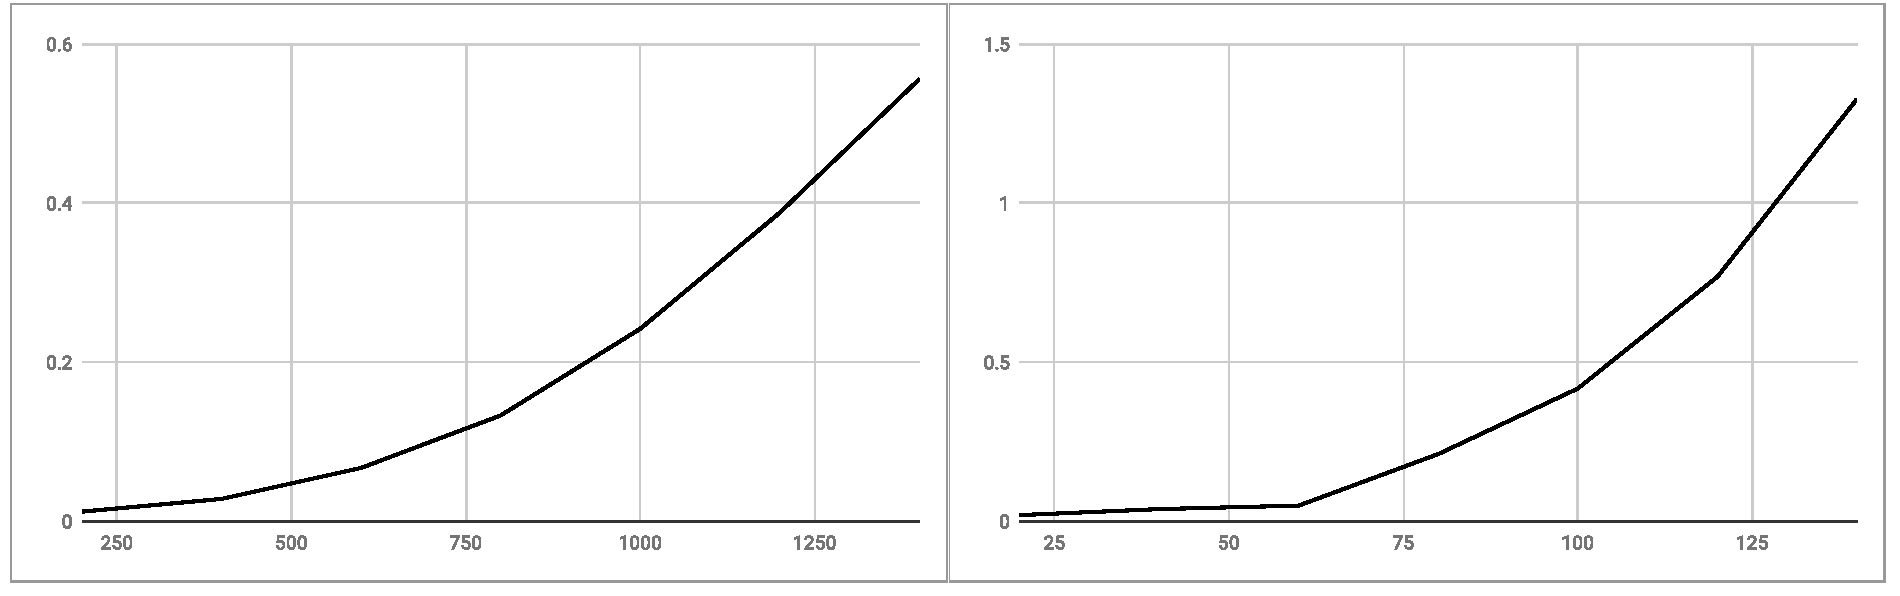
\includegraphics[width=15cm]{figure/graph.pdf}.
		\end{figure}

%%% Local Variables:
%%% mode: latex
%%% TeX-master: "../Report"
%%% End:
